\documentclass[10pt,a4paper]{article}
\usepackage[utf8]{inputenc}
\usepackage[T1]{fontenc}
\usepackage[spanish]{babel}
\usepackage{amsmath}
\usepackage{amsfonts}
\usepackage{amssymb}
\usepackage{graphicx}
\usepackage{float}
\usepackage{subcaption}
\usepackage[colorlinks=true, citecolor=blue, final]{hyperref}
\usepackage[table]{xcolor}
\usepackage{amsmath}
\usepackage{graphicx}
\usepackage{soul}
\usepackage{color}
\newcommand{\hilight}[1]{\colorbox{yellow}{#1}}
\usepackage{epstopdf}
\epstopdfDeclareGraphicsRule{.gif}{png}{.png}{convert gif:#1 png:\OutputFile}
\AppendGraphicsExtensions{.gif}
\usepackage{amssymb}
\setlength{\arrayrulewidth}{1mm}
\setlength{\tabcolsep}{18pt}
\renewcommand{\arraystretch}{2.5}
\usepackage{url} % UTILIZA EL PAQUETE PARA QUE APAREZCA EL URL AUNQUE AUN NOSE SI DEBO ACTIVARLO TAMBIEN EN REFERENCIAS
\hypersetup{
    colorlinks=true,
    linkcolor=blue,
    filecolor=blue,      
    urlcolor=blue,
}
\usepackage{epsfig}
\hypersetup{colorlinks=true,
    linkcolor=blue,
    filecolor=blue,      
    urlcolor=blue,}
\usepackage{graphicx}
\usepackage[sort&compress, numbers]{natbib}
\usepackage{xcolor}
\usepackage{listings}
\usepackage{ragged2e}
\definecolor{codegreen}{rgb}{0,0.6,0}
\definecolor{codegray}{rgb}{0.5,0.5,0.5}
\definecolor{codepurple}{rgb}{0.58,1,0.82}
\definecolor{backcolour}{rgb}{1,1,0.97}
\lstdefinestyle{mystyle}{
    backgroundcolor=\color{backcolour},   
    commentstyle=\color{codegreen},
    keywordstyle=\color{magenta},
    numberstyle=\tiny\color{codegray},
    stringstyle=\color{codepurple},
    basicstyle=\ttfamily\footnotesize,
    breakatwhitespace=false,         
    breaklines=true,                 
    captionpos=b,                    
    keepspaces=true,                 
    numbers=left,                    
    numbersep=0.4pt,                  
    showspaces=false,                
    showstringspaces=false,
    showtabs=false,                  
    tabsize=2
}
\lstset{style=mystyle}
\usepackage{lipsum}
\usepackage{multicol}
\usepackage{xcolor}
\newcommand{\celda}[1]{
	\begin{minipage}{2cm}
		\vspace{2mm}
		#1
		\vspace{2mm}
	\end{minipage}
}
\definecolor{azul}{rgb}{0.36, 0.54, 0.66}
\usepackage[left=2.00cm, right=2.00cm, top=2.00cm, bottom=2.00cm]{geometry}
\author{José Adrian Garcia fUENTES}
\begin{document}
	\begin{figure}[H]
		\raggedright
		\includegraphics[scale=0.5]{uanl (1).png} \hfill \includegraphics[scale=0.275]{fime.png}
	\end{figure}

	\vspace{6mm}
	
	%ESTE CENTER ES EXCLUSIVO PARA EL TITULO DEL PAPER, AUTOR Y UNIVER.
	\begin{center}
		{\Large \textbf{Práctica 3: Teoría de colas}}\\
		\vspace{2mm}
		\textit{ Alumno: José Adrian Garcia Fuentes}\\
		\textit{Profesor: Satu Elisa Schaeffer}\\
		\vspace{2.5mm}
		\textit{Universidad Autónoma de Nuevo León\hl{,} Facultad de Ingeniería Mecánica y Eléctrica\hl{ }}\\
		\vspace{1mm}
		\textit {\today}
		
		
	\end{center}
	\begin{center}
		\textcolor{azul}{\rule{150mm}{0.8mm}}
	\end{center}
	
	\vspace{5mm}

	\begin{multicols}{2}
		\section{Introducción} 
	La teoría de colas es un área de las matemáticas que estudia el comportamiento de líneas de espera. Los trabajos que están esperando ejecución en un \hl{cl\'uster} esencialmente forman una línea de espera \cite{p3}.

 

		\section{Objetivo} 
		Examinar cómo las diferencias en los tiempos de ejecución de los diferentes ordenamientos cambian cuando se varía el número de núcleos asignados al \hl{cl\'uster}, utilizando como datos de entrada un vector que contiene primos grandes, descargados de \url{https://primes.utm.edu/lists/small/millions/} y no primos (creados a partir de ellos)\hl{.} Con por lo menos nueve dígitos, aplicando pruebas estadísticas adecuadas y visualización científica clara e informativa \cite{p3}. 

\section{Metodología}
La metodología empleada se realizó a través de RStudio\cite{RStudio} llevando a cabo los pasos señalados en la \textit{Práctica 3: teoría de colas} \cite{p3}.\hl{ }

	
	\section{Resultados}
	Se obtuvo el código secuencia para determinar si un número es primo o no primo, a partir de este experimento se \hl{determin\'o} el tiempo que tardaba en detectar si era primo o no primo. \hl{El c\'odigo del experimento se encuentra en el repositorio de Garcia} \cite{gitadrian} en el cual se señala el número de repeticiones y parte de la función dada solicitando números de manera pseudoaleatoria, \hl{dicho c\'odigo fue modificado del c\'odigo del Schaeffer} \cite{p3gitdr}. 
	
	En la figura \ref{fig2} \hl{se muestra un diagrama de viol\'in de los tiempos de ejecuci\'on de cada orden (original, invertido y aleatorio) respectivamente, el tiempo en segundos es mayor para el orden original y menor para el invertido.}
	\vspace{1mm}
	
	\hl{En el cuadro} \ref{tb: Tabla1} \hl{se muestran los datos estad\'isticos de cada orden, se muestran valores muy similares en medias de los tiempos de ejecuci\'on, como tambi\'en en el tiempo m\'inimo  y una ligera diferencia en el tiempo m\'aximo.}

	
\begin{figure}[H]
				\centering
				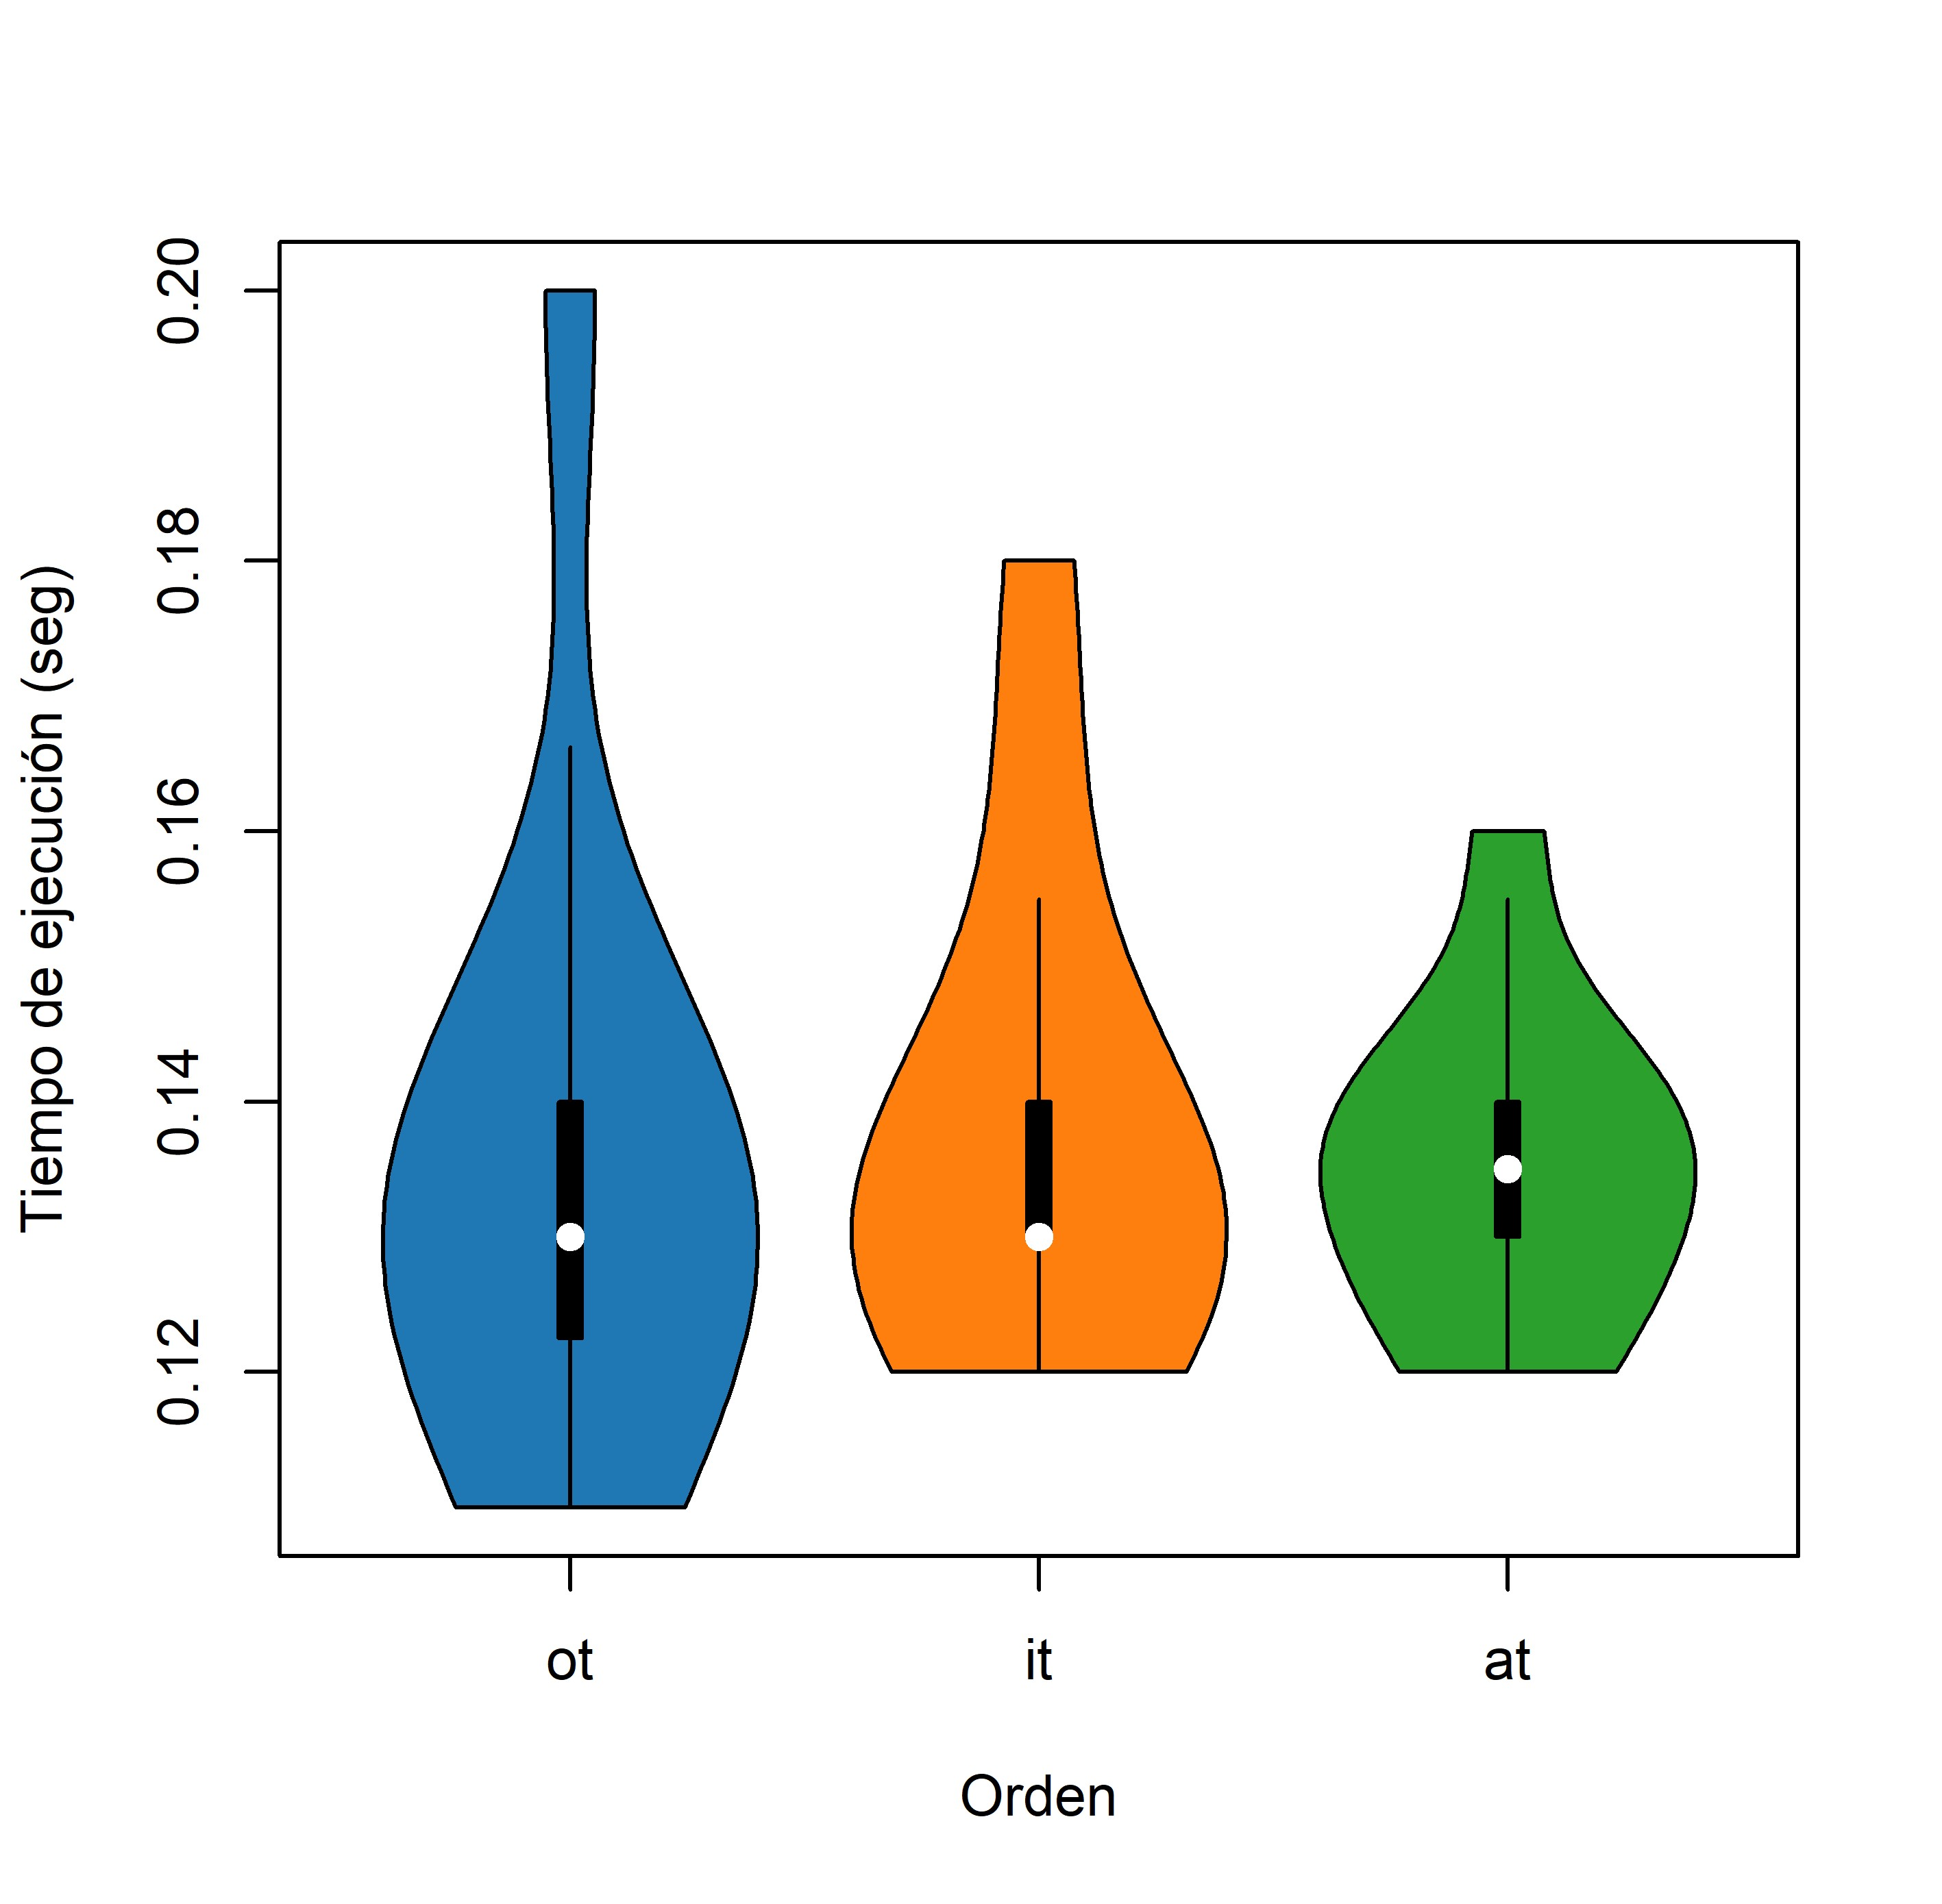
\includegraphics[scale=0.1]{3corregida.tif.jpg} 
				\caption{Tiempos de ejecución para cada orden.}
				\label{fig2}
\end{figure}


		\section{Conclusión}
		En conclusión el tiempo en que tarda un experimento en correr una secuencia variando el \hl{n\'umero} de \hl{n\'ucleos} de un \hl{CPU} puede ser \hl{m\'as} corto \hl{dependiendo} de que tan largo sea el experimento \hl{para el caso de los tiempos de ejecuci\'on de la figura} \ref{fig2} \hl{el orden con mayor tiempo fue el original con un m\'aximo de veinte segundos para el caso del orden aleatorio un m\'aximo de diecis\'eis segundos, el c\'odigo se encuentra en el repositorio de Garcia} \cite{gitadrian}, \hl{sin embargo al realizar modificaciones del c\'odigo se obtuvo un tiempo de ejecuci\'on mayor al esperado esto puede deberse a alg\'un error en la asignaci\'on del n\'umero de n\'ucleos o bien a la cantidad total procesada de n\'umeros primos.}
\end{multicols}
	\begin{table}[ht]
		\centering
		\caption{Descripción estadística}
		\begin{tabular}{|c|c|c|c|c|c|c|}
			\hline
			 Orden & Mín & $1$er. Q & Mediana & Media & $3$er Q & Máx \\
			\hline
			Original & $0.11$ & $0.12$ & $0.13$ & $0.13$ & $0.14$ & $0.20$ \\
			\hline
			Invertido& $0.12$ & $0.13$ & $0.13$ & $0.13$ & $0.14$ & $0.18$\\
			\hline
			Aleatorio & $0.12$ & $0.13$ & $0.13$ & $0.13$ & $0.14$ & $0.16$\\
			\hline
		\end{tabular}
	\label{tb: Tabla1}
	\end{table}
	
	\begin{multicols}{2}

\bibliography{T12}
	\end{multicols}
\bibliographystyle{ieeetr}
	
\end{document}
